\documentclass[a4paper, 11pt]{report}


\usepackage[utf8]{inputenc}
\usepackage{graphicx}
\usepackage{hyperref}
\usepackage{fancyhdr}
\graphicspath{ {./Figures/} }
\usepackage[table,xcdraw]{xcolor}
\usepackage{listings}
\usepackage{xcolor}

\definecolor{codegreen}{rgb}{0,0.6,0}
\definecolor{codegray}{rgb}{0.5,0.5,0.5}
\definecolor{codepurple}{rgb}{0.58,0,0.82}
\definecolor{backcolour}{rgb}{0.95,0.95,0.92}

\lstdefinestyle{mystyle}{
    backgroundcolor=\color{backcolour},   
    commentstyle=\color{codegreen},
    keywordstyle=\color{magenta},
    numberstyle=\tiny\color{codegray},
    stringstyle=\color{codepurple},
    basicstyle=\ttfamily\footnotesize,
    breakatwhitespace=false,         
    breaklines=true,                 
    captionpos=b,                    
    keepspaces=true,                 
    numbers=left,                    
    numbersep=5pt,                  
    showspaces=false,                
    showstringspaces=false,
    showtabs=false,                  
    tabsize=2
}

\lstset{style=mystyle}


\fancypagestyle{plain}{
  \fancyhf{}% Clear header/footer
  \rhead{John Montgomery - 5199}
\lhead{Kimberley College Sixth Form - 15125}
\lfoot{\thepage}
\rfoot{Robotron 2084: Pygame remake}
}
\pagestyle{plain}% Set page style to plain.

\title{%
    
    \begin{center}
        
\includegraphics[width=3cm]{kimberley.png}
        \centering
    \end{center}
  Robotron: 2084 inspired Game \\
  \large Written in PyGame with MVC architecture}
\author{{\Large John Montgomery}\\ \ 
Candidate Number: 5199\\
Centre Name: Kimberley College Sixth Form\\
Centre Number: 15125\\
Qualification: AQA 7517 (A--Level Computer Science)\\ \\
{\small Supervisor: B. Harris}}
\date{2020-2022}




\begin{document}

\maketitle

\newpage
\tableofcontents\thispagestyle{empty}
\newpage
\listoffigures\thispagestyle{empty}
\newpage
\chapter{Abstract}
    This project is a modernised version of robotron 2084, it has 2 sections, the game code and the website. The game code, which is a remake of Robotron 2084, a classic arcade game, this is backed with an MVC architecture which is designed to separate out the functionalities of the game and communicates with the website via an API. The website will use a database with multiple tables to store all the scores and logins and will also be used to display the high scores of users.

\chapter{Analysis}
\section{What is MVC?}
Model-View-Controller plays a large part in the project, the diagram [Figure \ref{fig:MVC_overview}] shows the main way that MVC works. It isolates the components of the game into 3 main components. The View, which is the screen, or what the user will see. The controller, which is where the user interacts with the game, in this case it is the interaction with the keyboard. The model, which is the part the user never interacts with, and stores the state of the game and current information about it.

\begin{figure}[h]
  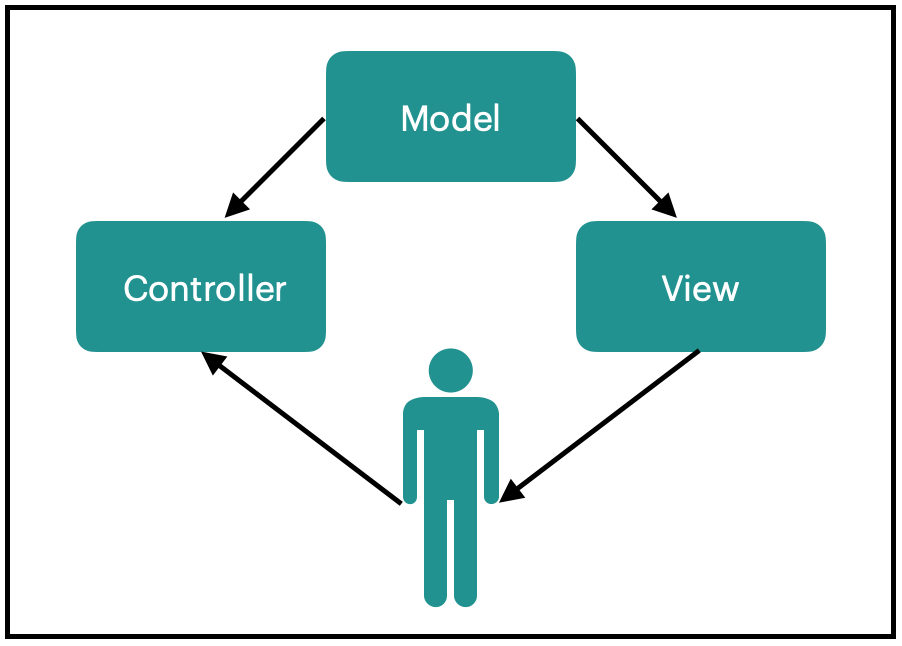
\includegraphics[width=\linewidth]{MVC overview.png}
  \caption{A diagram showing the MVC architecture}
  \label{fig:MVC_overview}
\end{figure}

There are many benefits to this set up, for example, it will easily allow me to swap out what controller is used. If desired, it is much simpler to replace the keyboard as the human interface, and replace it with a game controller. Even more useful may be the ability to remove the controller and view entirely, allowing for a streamlined game which an AI could learn how to play. This flexibility, along with ease of programming is what drew me to use MVC for the game.

Another important information is the way information travels between the 3 sections. This is done with events, and an event manager is responsible for maintaining the sending and receiving of events through the system. A similarly important section is the States, and state machine, which controls the current ‘state’ the game is in, that is to say what level is being played, or what screens should be shown, such as a loading or help screen.

\section{The Game}
“Robotron: 2084” was released in 1982 by Williams Electronics. It was revolutionary as a dual stick shooter, was high energy and loved by many. This is important to capture into the game, where I want it to have a similar feeling to the original game, with some modern twists. 

The game is about a species of ‘Robotrons’ created by humans in the year 2084, after realising their failings and created an advanced species. The goal is to save the humans (Mommies, Daddies and Mikeys), whilst fighting the robots, which have many kinds. The most basic are electrodes, which are static obstacles that kill on contact, but can be shot by players. The other basic enemy is the grunt, which is simply a basic soldier, which kills on contact, but moves towards the player.
There are some other robots that will be talked about and implemented later, but the details about them are less important. 

\section{Limitations}
The dual stick shooter nature means the player uses one joystick to move, and one joystick to shoot. This is difficult to implement well with a keyboard, but a simple setup which I am using is having WASD to move, and IJKL to shoot. Holding 2 keys diagonally at the same time will result it movement in an angle, allowing for shooting in 8 directions, and moving in 8 too.

Robotron is a fast fast game, I had to slow it down slightly in order to make it more playable on my laptop, and so it does feel somewhat different to the original. However by slowing it as I have I have made it a much smoother game to play.

\section{Objectives}
\begin{enumerate}
    \item Create basic playing ability
        \begin{enumerate}
            \item Player can move in 8 directions
            \item Player can shoot in 8 directions
            \item Players animation is correct for direction of travel
        \end{enumerate}
    \item Create basic enemies
        \begin{enumerate}
            \item Enemy is spawned in random position
            \item Enemy can move
            \item Enemy is animated
            \item Enemy kills players
        \end{enumerate}
    \item Create Loading Screens
        \begin{enumerate}
            \item Fuzzy loading screen
            \item 'All test' screen
            \item Home Screen
        \end{enumerate}
    \item Create levels and transitions
        \begin{enumerate}
            \item Player moves between levels
            \item Level transitions
            \item Player is invincible on load
        \end{enumerate}
    \item Create the API
    \item Create login system
        \begin{enumerate}
            \item Basic API sign up works
            \item GUI interactions with PyGame
        \end{enumerate}
    \item High Scores
        \begin{enumerate}
            \item Top 10
            \item Player Search
        \end{enumerate}
    \item Create sounds with Game
    \item Create scoring and score counter
    \item Create a life counter
    \item Automate testing on API and basic functions in PyGame
\end{enumerate}

\section{Design and Inspiration}
The design for all the game is heavily taken from the original game. I used many places to research this, but below is a selection of screenshots and videos which were used in the creation of the game.
\begin{figure}[h!]
  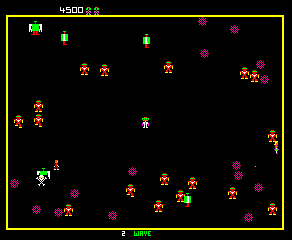
\includegraphics[width=0.8\linewidth]{design1.png}
  \centering
  \caption{Screen from original game - \url{https://arcadeblogger.com/2020/06/27/the-development-of-robotron/}}
  \label{fig:Design 1}
\end{figure}

\begin{figure}[h!]
  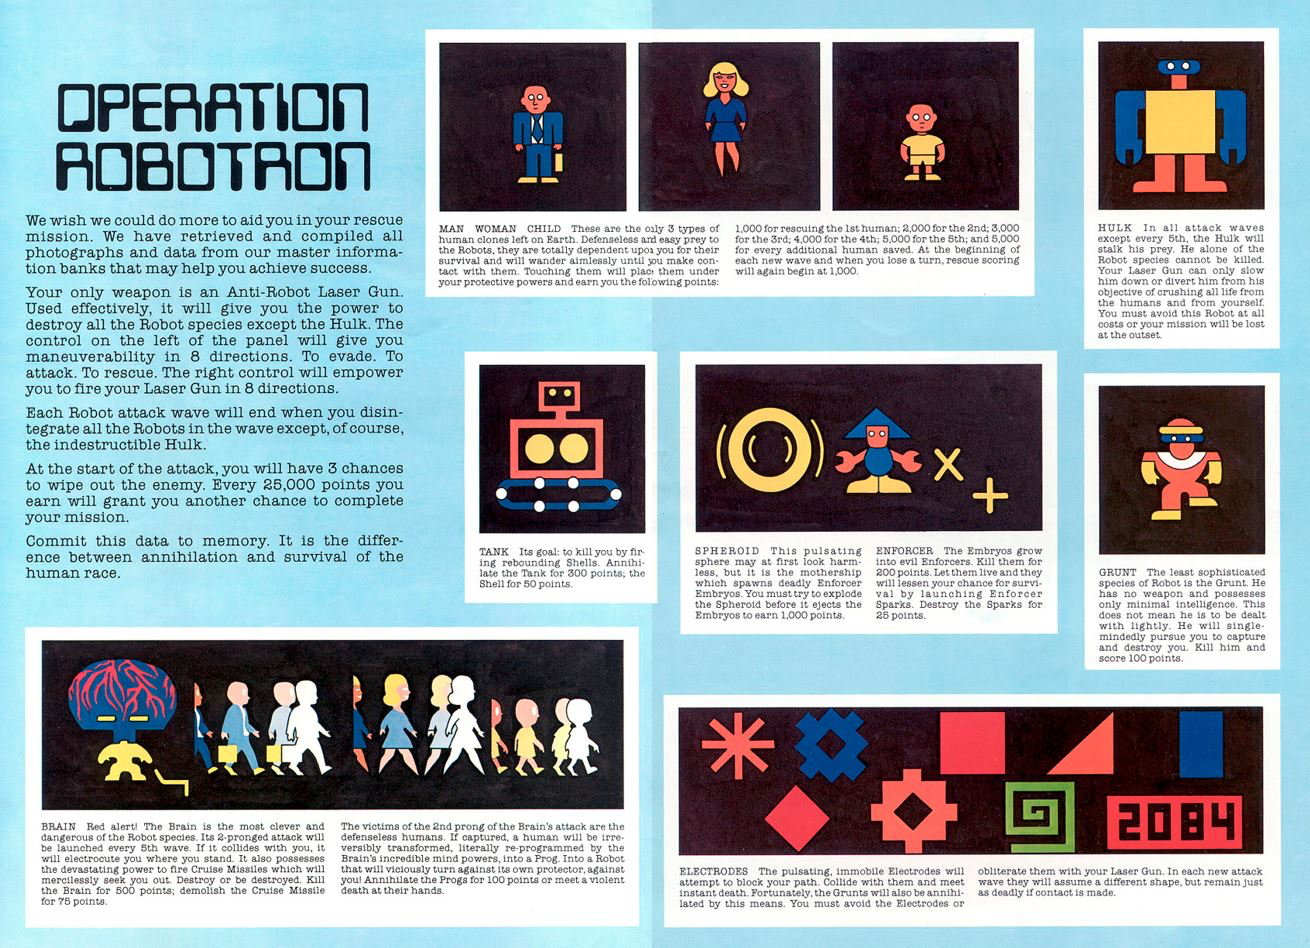
\includegraphics[width=0.8\linewidth]{design2.png}
  \centering
  \caption{Advertising Material - \url{https://arcadeblogger.com/2020/06/27/the-development-of-robotron/}}
  \label{fig:Design 1}
\end{figure}

\begin{itemize}
    \item \href{Video of screenplay, also useful to help create sound}{https://www.youtube.com/watch?v=ccltMtkFBSI}
    
    \item \href{Video of screenplay, also useful to help create sound}{https://www.youtube.com/watch?v=aOVA2Axxfdk}
\end{itemize}



\chapter{Documented Design}
The main design aspect is the MVC architecture and how it forms the basis of the game. Fig 1, from the analysis section, gave a very brief, high level and non technical view of MVC. In this section I will go into more detail about my own implementation, and how it works in greater detail. This section also details the database on the web side, the API, the technical setup of the servers, the data structures and HCI designs.

\section{MVC in practice}
In the analysis section I gave a very high level overview of MVC, this part will detail further into my design on its implementation in python. The first main, basic components of MVC are of course, the model, the view, and the controller. Figure \ref{fig:MVC_class} shows the 3 classes diagrams for each of the implementations of these in python.

\begin{figure}[h!]
  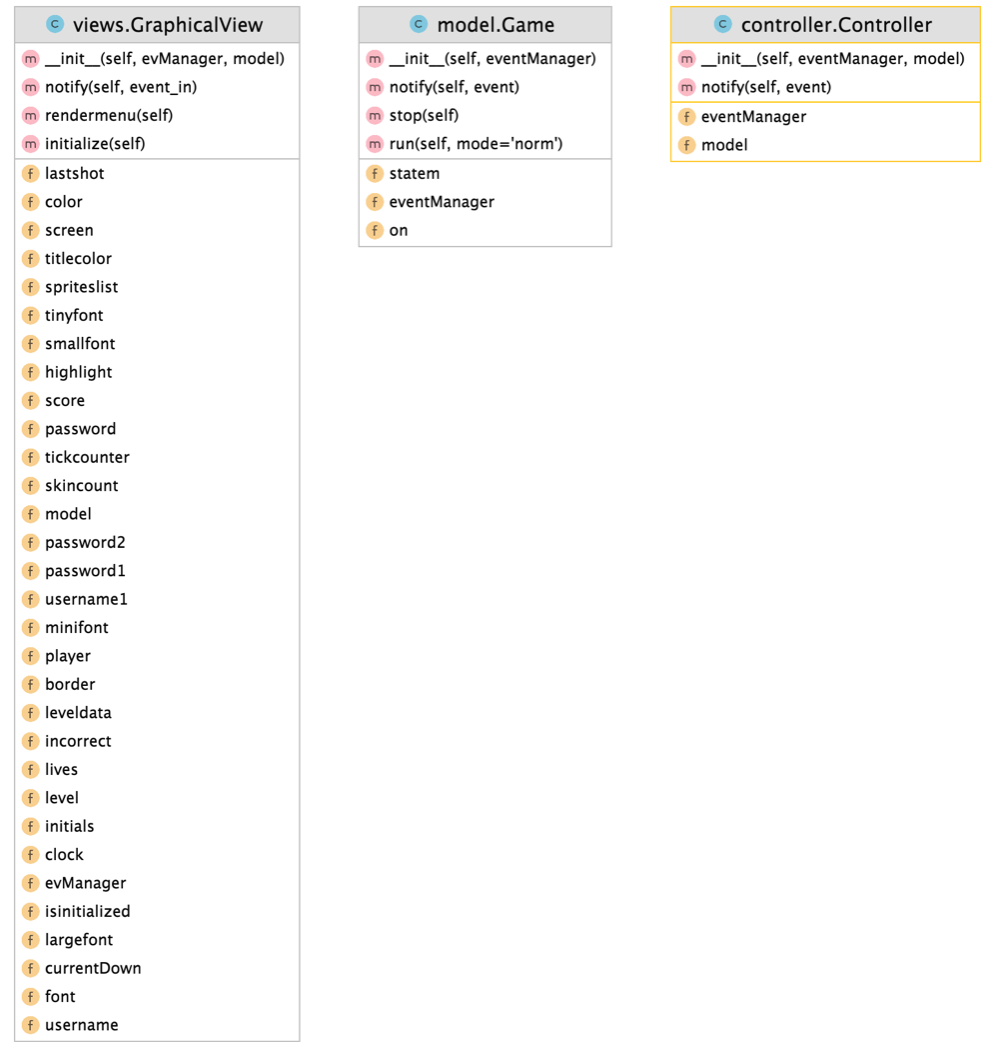
\includegraphics[width=0.8\linewidth]{mvc.png}
  \centering
  \caption{Class diagram}
  \label{fig:MVC_class}
\end{figure}

On top of these key features, there’s also a range of other important cogs in the system. One of the most important, to allow for the communication between the M, V and C are Events, and an event manager. A Sample of events, and the event manager is given in Fig {fig:events}.

\begin{figure}[h!]
  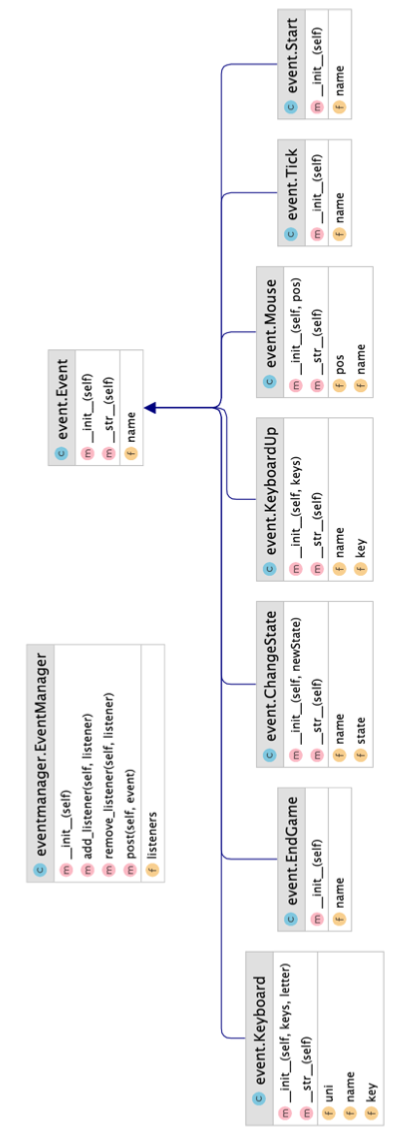
\includegraphics[height=0.8\linewidth, angle=270]{events.png}
  \centering
  \caption{Class diagram}
  \label{fig:events}
\end{figure}

The other key class is the state machine. Each state is not given its own class, rather there is a constant number which is attributed to a given state. The states are used for the larger changes in the program and events are for the smaller interactions, and ticks.
\begin{figure}[h!]
  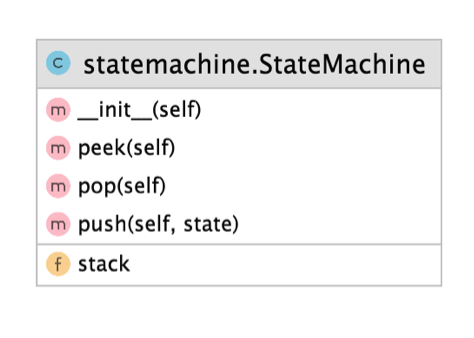
\includegraphics[width=0.8\linewidth]{state.png}
  \centering
  \caption{Class diagram}
  \label{fig:MVC_class}
\end{figure}

\begin{figure}[h!]
  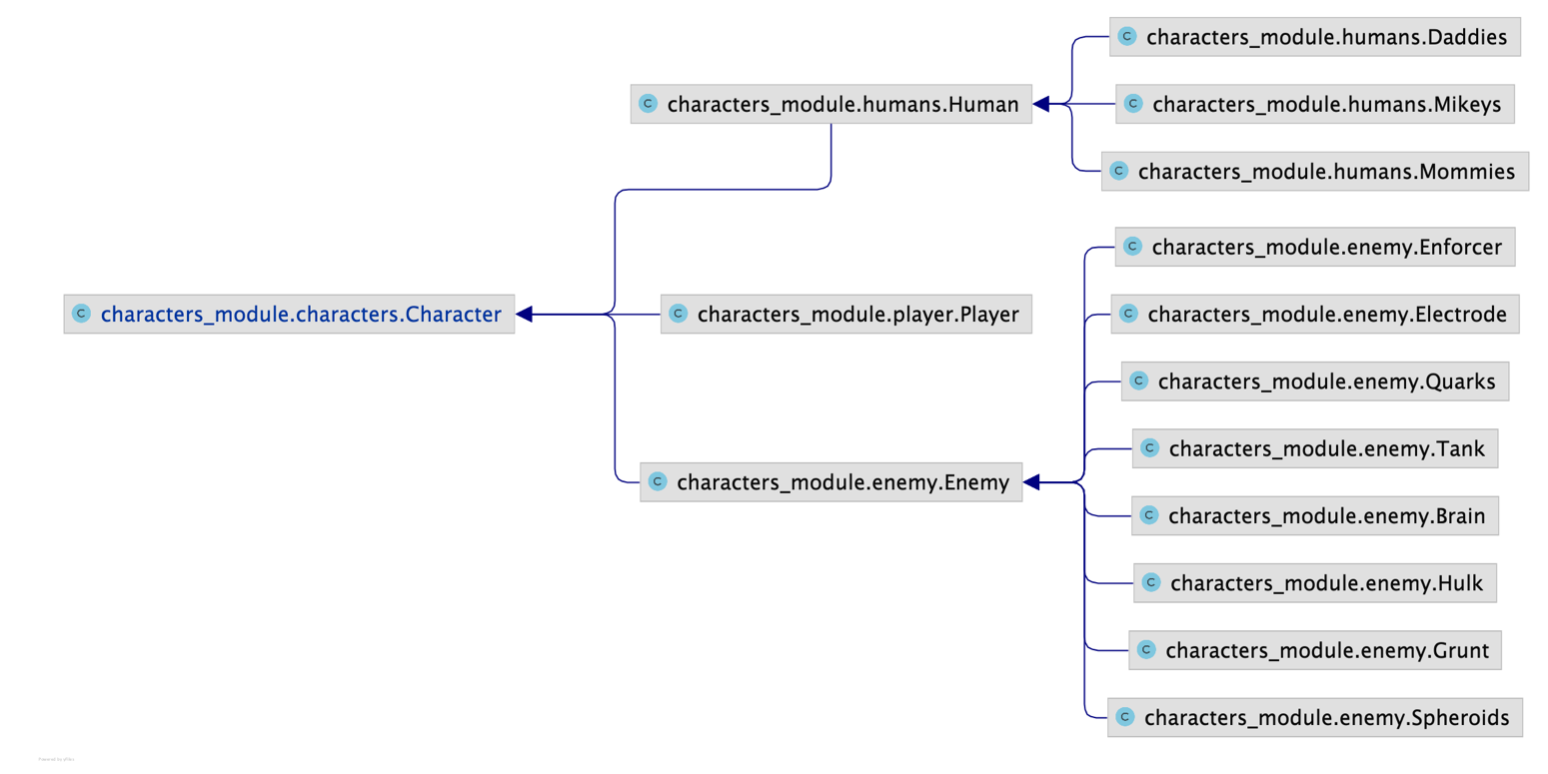
\includegraphics[width=0.8\linewidth]{class2.png}
  \centering
  \caption{Class diagram of characters}
  \label{fig:classeschars}
\end{figure}

\begin{figure}[h!]
  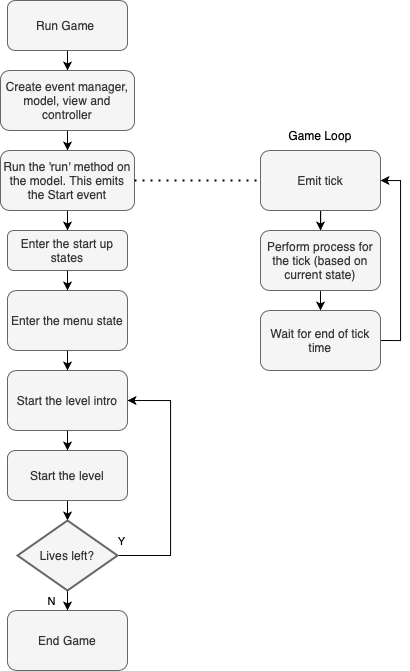
\includegraphics[width=0.8\linewidth]{flowchart}
  \centering
  \caption{Flowchart of MVC}
  \label{fig:flowchart}
\end{figure}

In order to run through a basic idea of what happens when the program is run, I have created a step by step flowchart. This flowchart [Fig 9] is a gross oversimplification, but works as a high level description of what it is my code is doing when executed.

\section{Database}
This section will show the database design and set up, and explain some of the SQL used in the program. Fig 10 shows the database diagram.


[TODO - Database diagram]


There are 3 tables, scores, users and tokens. The scores database has 2 fields which store the users ID and their Score for a given game. The Users table stores the users info, such as emails, password hashes, etc, and then the tokens database is used to store validated tokens (with time limits) which are used to validate the GUI and avoids needing to login to the the program every time the game is run. Fig 11 shows the process of creating the tokens.

\section{The API}
The leaderboard contains only 6 routes, as these were all that are necessary, the details for the routes are detailed in the table below.

\begin{figure}[h!]
  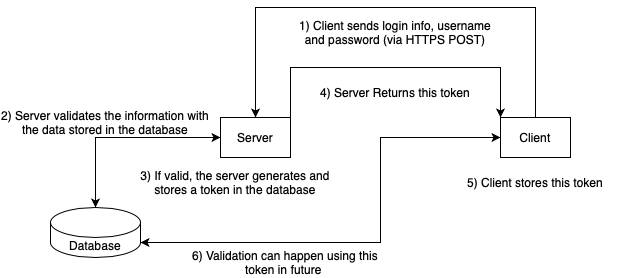
\includegraphics[width=0.8\linewidth]{tokens.png}
  \centering
  \caption{How tokens are generated}
  \label{fig:tokens}
\end{figure}

\begin{table}[h!]
\begin{tabular}{|l|l|l|}
\hline
\rowcolor[HTML]{C0C0C0} 
ROUTE            & METHOD & DESCRIPTION                                                  \\ \hline
/leaderboard     & GET    & Returns JSON of top 10 users (initials + scores) in Database \\ \hline
/user/userid     & GET    & Returns JSON of top score                                    \\ \hline
/username/userid & GET    & Returns ID of given username                                 \\ \hline
/login           & POST   & Logs in a user, sends token, or logs user in with token      \\ \hline
/addscore        & POST   & Adds a score, given score and a token                        \\ \hline
/adduser         & POST   & Adds a user to the database                                  \\ \hline
\end{tabular}
\end{table}


\section{The Server Setup}
Fig 12 shows the set up the server is in. All using AWS, there is an RDS Postgres database, and EC2 instance (this is the server running the actual flask) and then an S3 bucket to handle sending the static files. It may also be possible to use NGINX or Apache to serve and handle the API. This system may end up being better, so my current architecture could change. 

\section{Security}
Because the database and client handles personal details like email and passwords, there needs to be a thought to security. First off, there is an enforcement of passwords and a strong policy. Users passwords will need to be 8 characters, with 1 special, and my plan is to check them against a list of common passwords (rocky.txt) using hashes. For this I will probably use MD5, or something even faster. However it is important to avoid these fast algorithms when hashing passwords for storage. As such, passwords will undergo key derivation through bcrypt, an algorithm which not only salts, but performs many rounds of hashing. I could implement a similar algorithm using the basic functions like SHA, but rolling your own crypto is never good, so its going to be done with bcrypt, as this is essentially the best option available, and more than secure enough.

To help further security, HTTPS is being used for all the sending and receiving of data, this avoids man in the middle attacks of the data as it gets sent over the internet. 


\chapter{Technical Solution}
Im working on a way to easily do this. I am using LaTeX as this will allow me to not have to change the code on my report manually, as it will link to the files. However i am still learning. This file will also update on my github, so if you go to https://github.com/john-montgomery2003/Robotron2084 you will be able to find a pdf of this document which is more up to date.

\section{Example}

\chapter{Testing - TODO}
\chapter{Evaluation - TODO}
\chapter{Appendix \& Bibliography}
\section{Appendix}
\begin{table}[h!]
\begin{tabular}{|l|l|l|}
\hline
\rowcolor[HTML]{C0C0C0} 
{\color[HTML]{000000} \textbf{Name}} & {\color[HTML]{000000} \textbf{Server/Web/Game/Dev}} & {\color[HTML]{000000} \textbf{Use}}             \\ \hline
Flask                                & Server                                              & Handles the API and web on server side          \\ \hline
SQLalchemy                           & Server                                              & Used to connect to the Postgres database        \\ \hline
BCrypt                               & Server                                              & Key derivation                                  \\ \hline
Waitress                             & Server                                              & WSGI server                                     \\ \hline
PyGame                               & Game                                                & Graphics and input handling                     \\ \hline
S3                                   & Server                                              & AWS static file hosting / serving               \\ \hline
EC2                                  & Server                                              & AWS server to run flask app                     \\ \hline
Hetzner                              & Server                                              & Alternative option to run flask and serve files \\ \hline
PyCharm                              & Dev                                                 & My IDE choice                                   \\ \hline
\end{tabular}
\end{table}

\section{Listings}
\listoflistings


\end{document}

